\documentclass[10 pt]{report}   	% use "amsart" instead of "article" for AMSLaTeX format
\usepackage{amsmath}
\usepackage{amssymb}
\usepackage{float}
\usepackage[T1]{fontenc}
\usepackage{graphicx}
\usepackage[utf8]{inputenc}
\usepackage{mathtools}
\usepackage{wasysym}
\usepackage[paperheight = 29.7cm,paperwidth = 21.59cm,left = 3.81cm,right = 2.54cm,top = 2.54cm,bottom = 2.54cm]{geometry}                		% See geometry.pdf to learn the layout options. There are lots.
\geometry{letterpaper}    
\usepackage{graphicx}	
\usepackage{xurl}
\setlength\parindent{0pt}
\renewcommand{\arraystretch}{1.3}               		% ... or a4paper or a5paper or ... 
%\geometry{landscape}                		% Activate for rotated page geometry
%\usepackage[parfill]{parskip}    		% Activate to begin paragraphs with an empty line rather than an indent
			% Use pdf, png, jpg, or eps§ with pdflatex; use eps in DVI mode
								% TeX will automatically convert eps --> pdf in pdflatex		

%SetFonts

%SetFonts


%\title{Brief Article}
%\author{The Author}
%\date{}							% Activate to display a given date or no date

\begin{document}
%\maketitle
%\section{}
%\subsection{}
 \vspace{1\baselineskip}
 \begin{center}
 {\LARGE \textbf {CS 520: INTRO TO ARTIFICIAL INTELLIGENCE}}
 \end{center}
 
 \begin{center}
 {\LARGE \textbf {\\PROJECT 2}}
 \end{center}

 \vspace{1\baselineskip}
 \begin{center}
 {\Large \textbf {FACE AND DIGIT CLASSIFICATION}
 \end{center}
 
  \begin{center}
 {\Large  \\ \\December 08, 2022}
 \end{center}
 
 \vspace{1\baselineskip}
 \begin{center}
 {\Large\\Manasvini Nittala (Net ID: mn777)\\}
 \end{center}

 \begin{center}
 {\Large \\Sahithi Reddy Sakinala (Net ID: ss4362)\\}
 \end{center}
 
  \begin{center}
 {\Large \\Jahnavi Manchala (Net ID: jm2658)\\ \\ \\}
 \end{center}

\vspace(\baselineskip = 1 \baselineskip}
{\Large \textbf {\\ \\1. NAIVE BAYES\\ \\}}

\large {\\ \\\textbf {(A) ALGORITHM DESCRIPTION} \\ \\
In Naive Bayes, the feature used was pixel occupancy per region. So first, the algorithm finds the maximum pixel occupancy across all features and all pictures for that training set. With that maximum, it sets up a matrix for each unique data point (faces/not faces, 1,2,3, etc.). \\ \\
Each row corresponds to a feature, and each column is a number between 0 and count. Where count is nothing but the max value in that column. Next, the algorithm tallies and plots the feature and pixel data received from the training data in their corresponding matrix. So, for example, if the face picture had 9 pixels in region 1. The face matrix would add a +1 to row 1, column 9. Then at the end, it would divide each cell by
the total number of pictures to create percentages for each feature and pixel combination.\\ \\
Lastly, when you test, the algorithm will take the features from the testing image and look up the associated percent across all matrices. Each matrix will keep a score by multiplying each feature percent by each other as given by the testing image feature. Each matrix score is independent of the other. The prediction list will be chosen as the highest percentage of all the matrices. \\ \\ \\ \\ \\ \\
\textbf{(B) CHALLENGES FACED} \\ \\ 
1. Feature Extraction: Finding the right set of features was a bit difficult. \\ We first took the binary values as pixels but were unable to achieve the desired accuracy, so we split the binary array into grids. We tested by splitting into 5 x 5, 10 x 10, and 20 x 20 grids. We felt that 10 x 10 grids were pretty comfortable to work with. \\ \\ 

2. Unused Values: We first filled all our arrays like faces, not faces, and digits with 0s but later realized that they affected the final prediction array as we multiplied the probabilities. We solved it by replacing 0 with 0.01, small enough to be ignored but large enough to uphold the predictions. \\ 

\textbf{(C) TRAINING AND OBSERVATIONS} \\ \\
Observations for the Naive Bayes algorithm are based on its mean accuracy, standard deviation, prediction error, and time taken over 10\%\ to 100\%\ training samples. \\ \\
\textbf{i) Accuracy}
\begin{figure} [H]
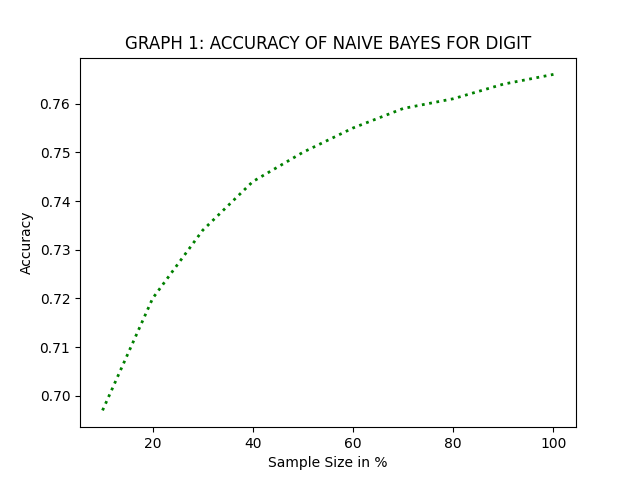
\includegraphics [width = 11cm, height = 8cm]{NB_ACC_DIGIT.png}
\end {figure}
\begin{center}
\small \textbf {Graph 1:} Mean Accuracy for Digit using Naive Bayes\\
\end{center}
\begin{figure} [H]
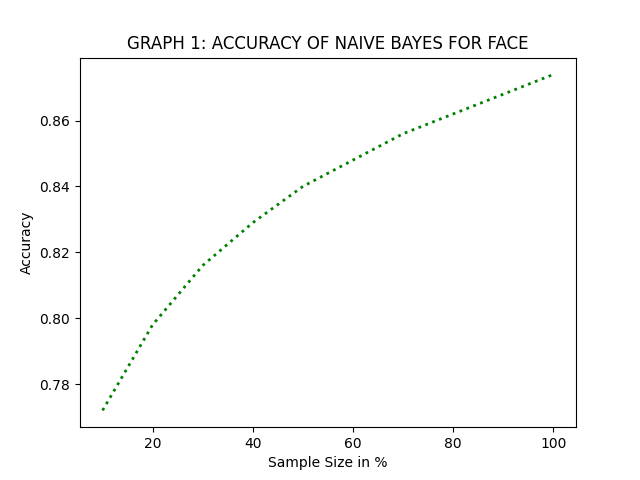
\includegraphics [width = 11cm, height = 8cm]{NB_ACC_FACE.png}
\end {figure}
\begin{center}
\small \textbf {Graph 2:} Mean Accuracy for Face using Naive Bayes\\
\end{center}
\textbullet\ As observed from the graphs, the Accuracy for both face and digit classification is increasing with an increase in the sample size. Maximum Accuracy for Digit was 77\%\ and for Face was 88\%\ \\  \\
\textbf{ii) Standard Deviation}
\begin{figure} [H]
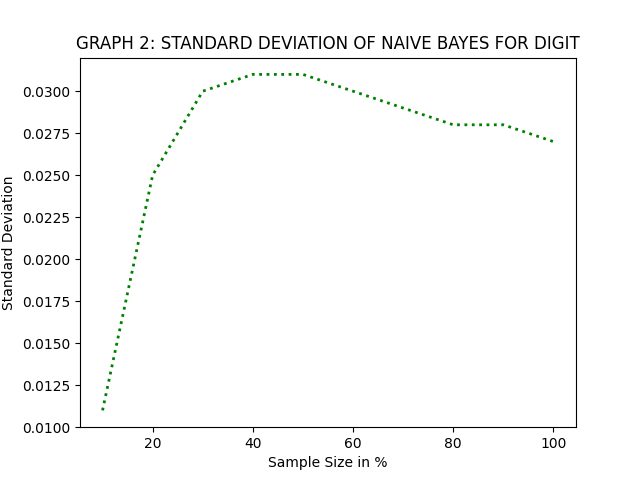
\includegraphics [width = 11cm, height = 8cm]{NB_STD_DIGIT.png}
\end {figure}
\begin{center}
\small \textbf {Graph 3:} Standard Deviation for Digit using Naive Bayes\\
\end{center}
\begin{figure} [H]
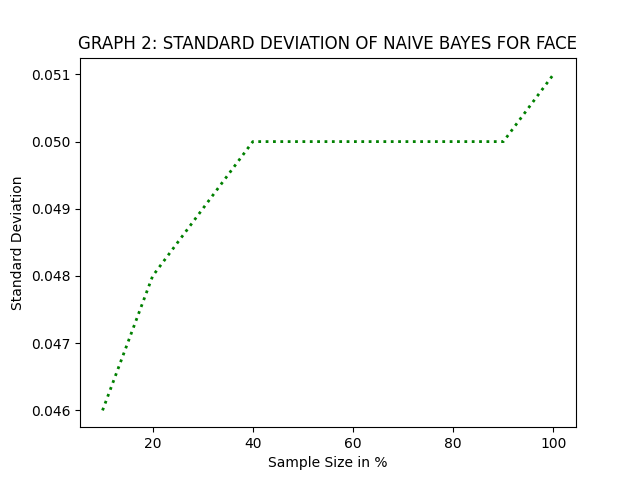
\includegraphics [width = 11cm, height = 8cm]{NB_STD_FACE.png}
\end {figure}
\begin{center}
\small \textbf {Graph 4:} Standard Deviation for Face using Naive Bayes\\
\end{center}
\textbullet\ As observed from the graphs, the Standard Deviation for both face and digit classification is increasing up to approximately 40\%\ samples but remains almost constant afterward. \\ \\
\textbf{iii) Time Taken}
\begin{figure} [H]
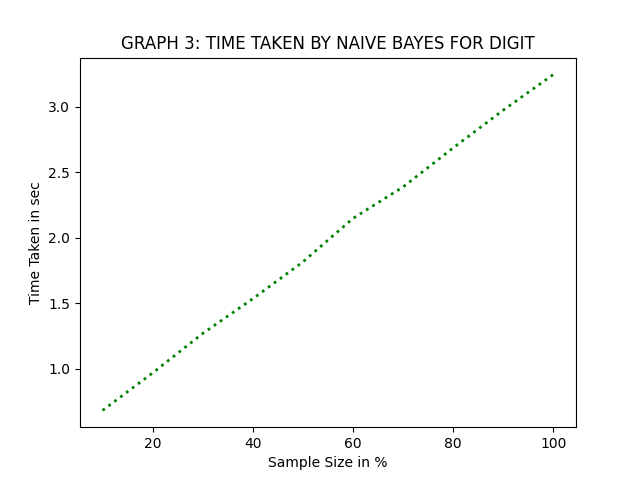
\includegraphics [width = 11cm, height = 8cm]{NB_TIME_DIGIT.png}
\end {figure}
\begin{center}
\small \textbf {Graph 5:} Time Taken for Digit using Naive Bayes\\
\end{center}
\begin{figure} [H]
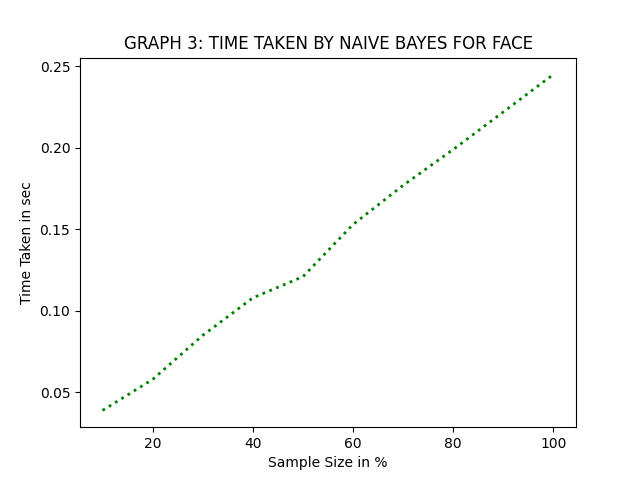
\includegraphics [width = 11cm, height = 8cm]{NB_TIME_FACE.png}
\end {figure}
\begin{center}
\small \textbf {Graph 6:} Time Taken for Face using Naive Bayes\\
\end{center}
\textbullet\ As observed from the graphs, the Time Taken for both face and digit classification has a linear relationship with the sample size. As the sample size increases, the time taken increases.\\ \\
\textbf{iv) Prediction Error}
\begin{figure} [H]
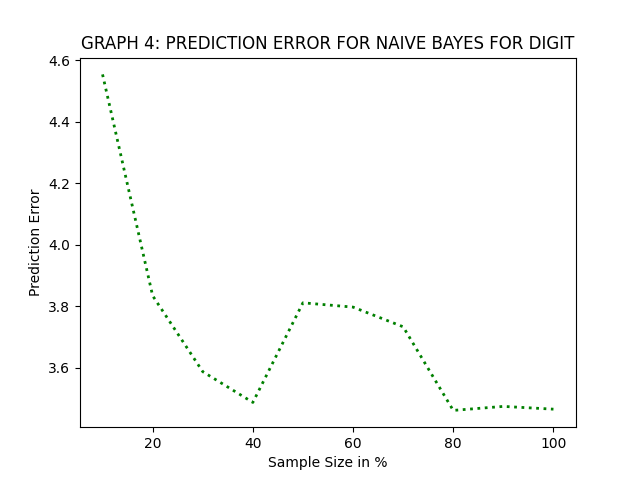
\includegraphics [width = 11cm, height = 8cm]{NB_PRED_DIGIT.png}
\end {figure}
\begin{center}
\small \textbf {Graph 7:} Prediction Error for Digit using Naive Bayes\\
\end{center}
\begin{figure} [H]
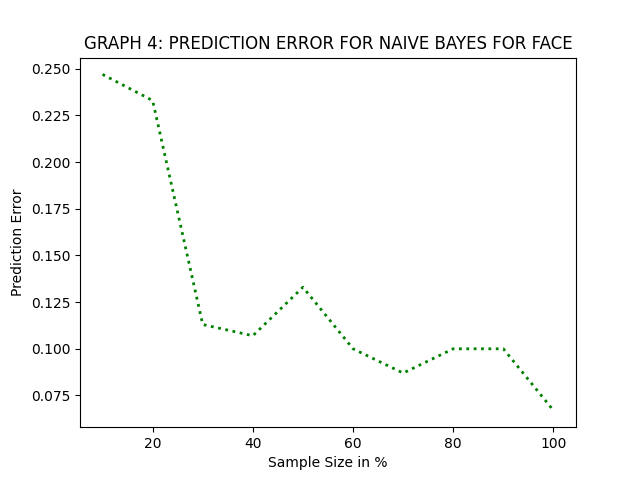
\includegraphics [width = 11cm, height = 8cm]{NB_PRED_FACE.png}
\end {figure}
\begin{center}
\small \textbf {Graph 8:} Prediction Error for Face using Naive Bayes\\
\end{center}
\textbullet\ As observed from the graphs, the prediction error for Digit is the root mean squared error (RMSE) between the actual test labels and the predicted test labels. As the sample size increases, the prediction error decreases. The prediction error for Face is the ratio of wrong predictions to the total number of predictions. For Face, too the prediction error decreases as the sample size increases.
}

{\Large \textbf {\\ \\2. PERCEPTRON\\ \\}}

\large {\\ \\\textbf {(A) ALGORITHM DESCRIPTION} \\ \\
This algorithm begins with initializing random weights for each feature, which We defined as pixel occupancy per region. We split the image into a 10x10 grid, so We have 100 features. Each image has 100 weights. The weight vector is calculated by multiplying each weight by its corresponding feature pixel density. 
If this resulting number is favorable for faces, then the image predicts that it is a face. \\ \\
If it is negative, then the prediction is not a face. To validate the correctness of the prediction, the algorithm checks the corresponding training label. 
If the prediction is correct, the algorithm moves on to the next image and calculates the weight vector again. If the prediction is too high (predicted face and it is not face), then each weight for that image is decremented by its corresponding feature. If the prediction is too low (predicted not face, and it is a face), then each weight is incremented by its corresponding feature. Our algorithm continues to loop through the training data and update the weights until it hits a threshold of 74\%\ correct guesses for digits and 81\%\ for faces. \\ 

The only difference between training faces and digits is that for each image, the algorithm calculates the weight vector for the digits 1-9 and chooses the highest one for its prediction.
If the prediction is wrong, the weights for the wrong predicted digit are decreased by their respective features, and the weights for the correct digit are increased by their respective features. This process takes quite a long time due to the number of calculations that must be
made at each iteration.\\ \\ 
\textbf{(B) CHALLENGES FACED} \\ \\ 
The main challenge in implementing perceptron is how much longer it took to train digits rather than faces since guessing a face is a binary decision, while digits are not. Also, calculating each f(x) weight vector for the digits took longer than calculating just one f(x) weight vector for faces. This takes up more run time as well as memory.\\ \\
\textbf{(C) TRAINING AND OBSERVATIONS} \\ \\
Observations for the Naive Bayes algorithm are based on its mean accuracy, standard deviation, prediction error, and time taken over 10\%\ to 100\%\ training samples. \\ \\
\textbf{i) Accuracy}
\begin{figure} [H]
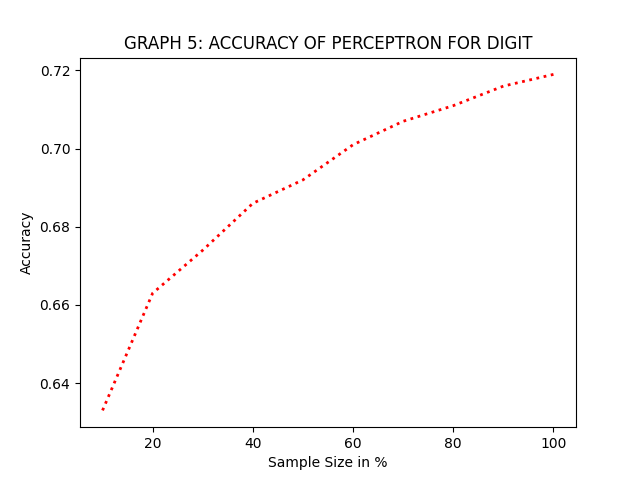
\includegraphics [width = 11cm, height = 8cm]{PERC_ACC_DIGIT.png}
\end {figure}
\begin{center}
\small \textbf {Graph 9:} Mean Accuracy for Digit using Perceptron\\
\end{center}
\begin{figure} [H]
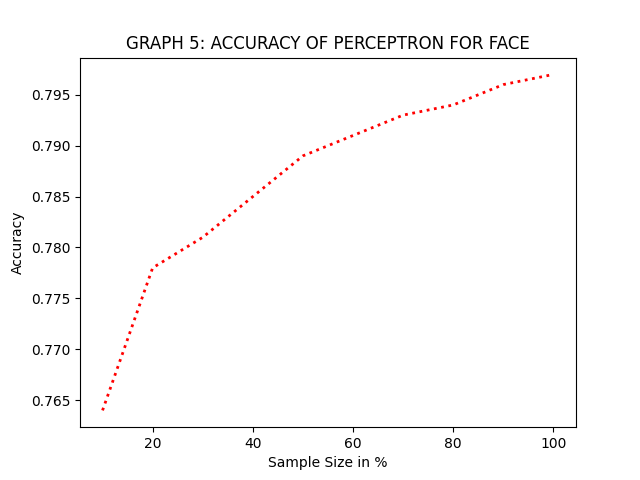
\includegraphics [width = 11cm, height = 8cm]{PERC_ACC_FACE.png}
\end {figure}
\begin{center}
\small \textbf {Graph 10:} Mean Accuracy for Face using Perceptron\\
\end{center}
\textbullet\ As observed from the graphs, the Accuracy for both face and digit classification is increasing with an increase in the sample size. Maximum Accuracy for Digit was 72\%\ and for Face was 81\%\ \\  \\
\textbf{ii) Standard Deviation}
\begin{figure} [H]
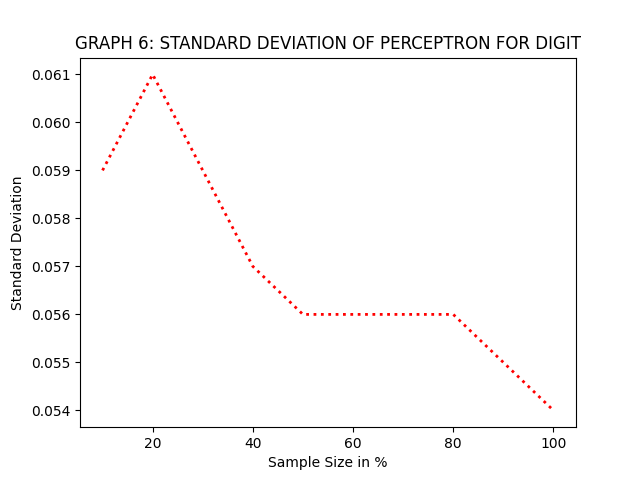
\includegraphics [width = 11cm, height = 8cm]{PERC_STD_DIGIT.png}
\end {figure}
\begin{center}
\small \textbf {Graph 11:} Standard Deviation for Digit using Perceptron\\
\end{center}
\begin{figure} [H]
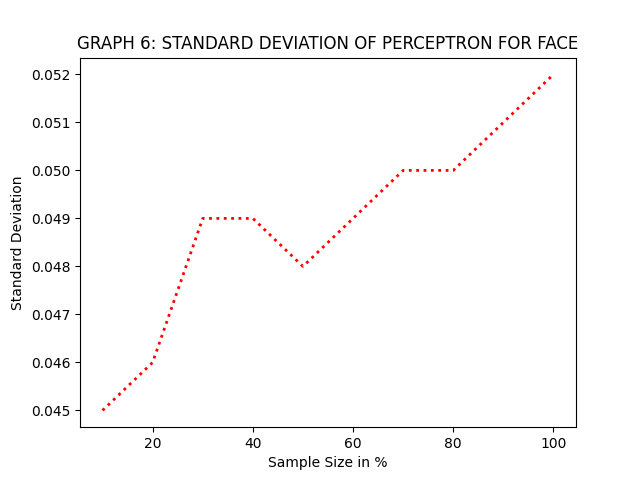
\includegraphics [width = 11cm, height = 8cm]{PERC_STD_FACE.png}
\end {figure}
\begin{center}
\small \textbf {Graph 12:} Standard Deviation for Face using Perceptron\\
\end{center}
\textbullet\ As observed from the graphs, the Standard Deviation for Digit is seeing a decreasing trend as the sample size increases whereas Face is seeing an increasing trend but we should make an observation that these standard deviation values are very very close and can be approximated to one value.\\ \\
\textbf{iii) Time Taken}
\begin{figure} [H]
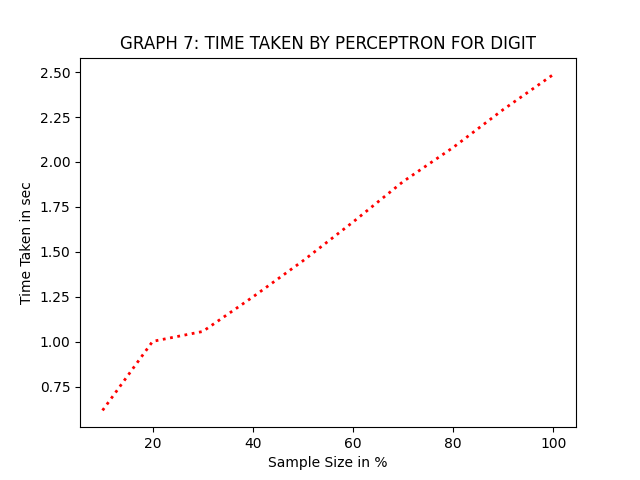
\includegraphics [width = 11cm, height = 8cm]{PERC_TIME_DIGIT.png}
\end {figure}
\begin{center}
\small \textbf {Graph 13:} Time Taken for Digit using Perceptron\\
\end{center}
\begin{figure} [H]
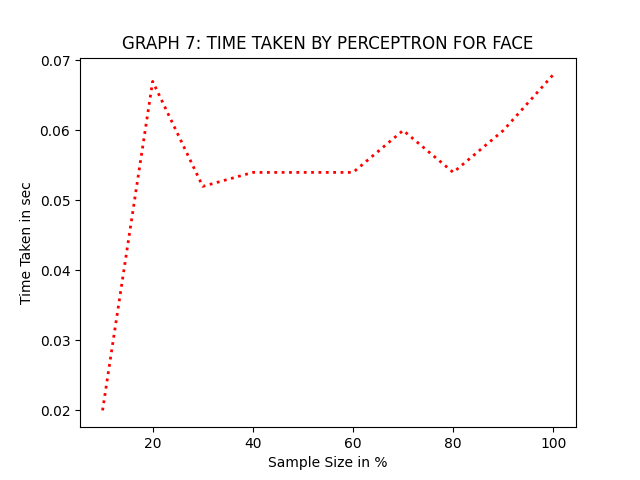
\includegraphics [width = 11cm, height = 8cm]{PERC_TIME_FACE.png}
\end {figure}
\begin{center}
\small \textbf {Graph 14:} Time Taken for Face using Perceptron\\
\end{center}
\textbullet\ As observed from the graphs, the Time Taken for both face and digit classification has an almost linear relationship with the sample size. As the sample size increases, the time taken increases.\\ \\
\textbf{iv) Prediction Error}
\begin{figure} [H]
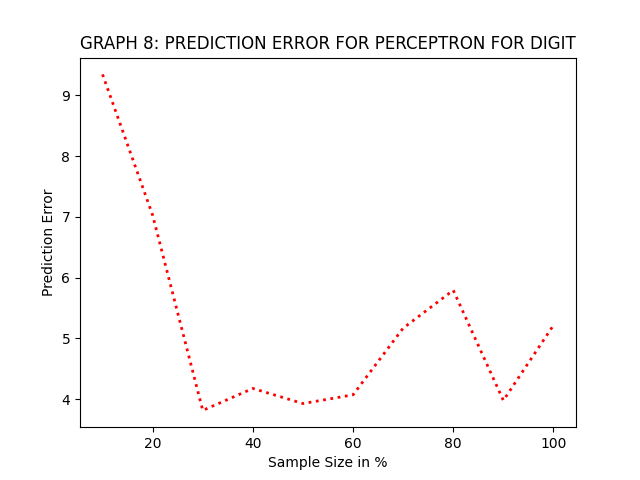
\includegraphics [width = 11cm, height = 8cm]{PERC_PRED_DIGIT.png}
\end {figure}
\begin{center}
\small \textbf {Graph 15:} Prediction Error for Digit using Perceptron\\
\end{center}
\begin{figure} [H]
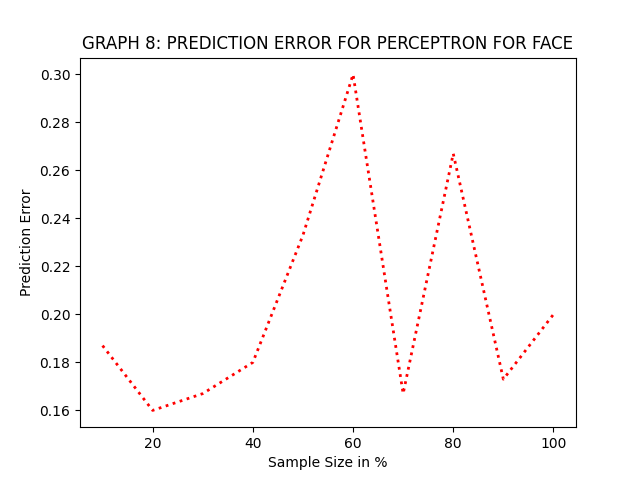
\includegraphics [width = 11cm, height = 8cm]{PERC_PRED_FACE.png}
\end {figure}
\begin{center}
\small \textbf {Graph 16:} Prediction Error for Face using Perceptron\\
\end{center}
\textbullet\ {As observed from the graphs, the prediction error for Digit is the root mean squared error (RMSE) between the actual test labels and the predicted test labels. As the sample size increases, the prediction error decreases. The prediction error for Face is the ratio of wrong predictions to the total number of predictions. For Face, many fluctuations are observed, but when trained with 100\%\ training data, the prediction error is the minimum.}
}
{\Large \textbf {\\ \\3. k NEAREST NEIGHBORS\\ }

\large {\\ \\\textbf {(A) ALGORITHM DESCRIPTION} \\ 

This algorithm works by taking the euclidean distance of the features in the testing image against all the features of the images in the training data. So, for example, image 1 of the testing data would be compared against all 5000 images in the training data by finding the euclidean distance for each pairing. 
Then all that data is saved into an array and sorted from lowest to highest. After that, the first three cells are chosen to vote. The most frequently seen within those three cells is chosen for the predictions. This process repeats for each image in the
training set. \\ \\ 
\textbf{(B) CHALLENGES FACED} \\ \\ 
1. Run Time: The main challenge we faced while implementing kNN was the time it took to return predictions. This problem arose with Digit data as there need to be 5000 comparisons made, and we are also iterating it to get the mean values. We have tried other methods instead but found the comparison to be the best way. We have reduced the run time by decreasing the number of iterations.\\ \\ 

\textbf{(C) TRAINING AND OBSERVATIONS} \\ \\
Observations for the Naive Bayes algorithm are based on its mean accuracy, standard deviation, prediction error, and time taken over 10\%\ to 100\%\ training samples. \\ \\
\textbf{i) Accuracy}
\begin{figure} [H]
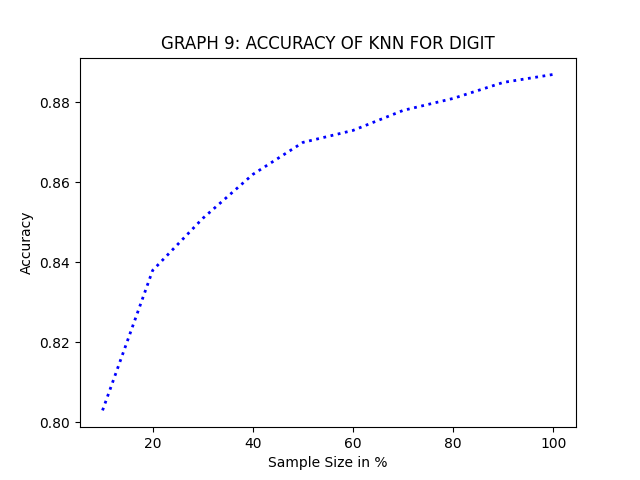
\includegraphics [width = 11cm, height = 8cm]{KNN_ACC_DIGIT.png}
\end {figure}
\begin{center}
\small \textbf {Graph 17:} Mean Accuracy for Digit using kNN\\
\end{center}
\begin{figure} [H]
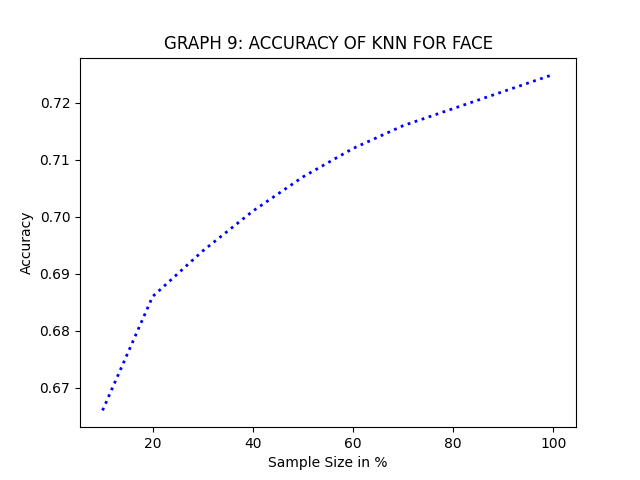
\includegraphics [width = 11cm, height = 8cm]{KNN_ACC_FACE.png}
\end {figure}
\begin{center}
\small \textbf {Graph 18:} Mean Accuracy for Face using kNN\\
\end{center}
\textbullet\ As observed from the graphs, the Accuracy for both face and digit classification is increasing with an increase in the sample size. Maximum Accuracy for Digit was 88\%\ and for Face was 74\%\ \\  \\
\textbf{ii) Standard Deviation}
\begin{figure} [H]
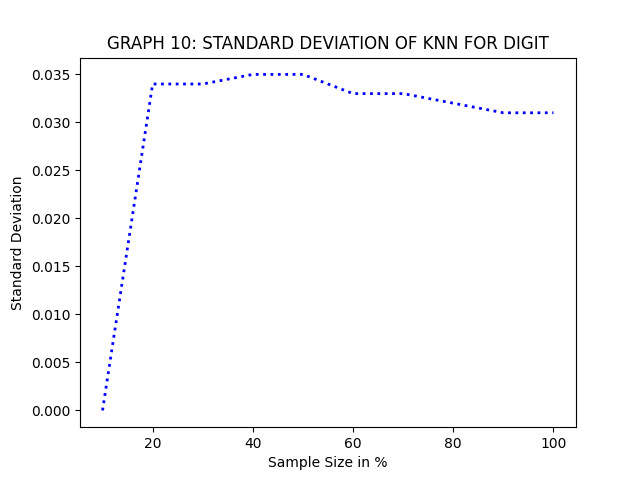
\includegraphics [width = 11cm, height = 8cm]{KNN_STD_DIGIT.png}
\end {figure}
\begin{center}
\small \textbf {Graph 19:} Standard Deviation for Digit using kNN\\
\end{center}
\begin{figure} [H]
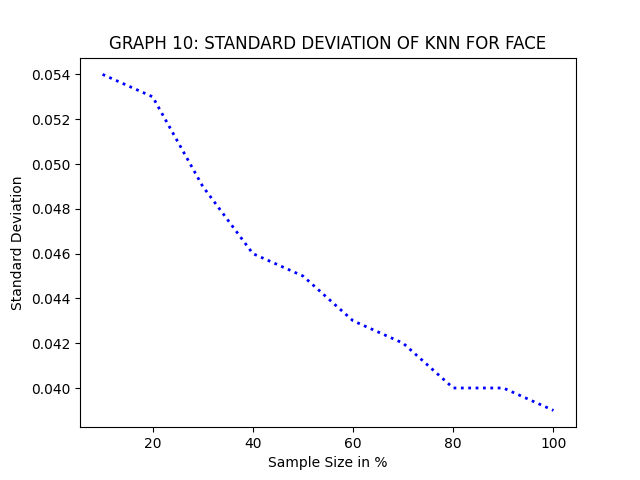
\includegraphics [width = 11cm, height = 8cm]{KNN_STD_FACE.png}
\end {figure}
\begin{center}
\small \textbf {Graph 20:} Standard Deviation for Face using kNN\\
\end{center}
\textbullet\ As observed from the graphs, the Standard Deviation for digit classification increases up to approximately 20\%\ samples but remains almost constant afterward, but for Face data, there is a decreasing trend observed, whereas the sample size increases the standard deviation is decreasing. \\ \\
\textbf{iii) Time Taken}
\begin{figure} [H]
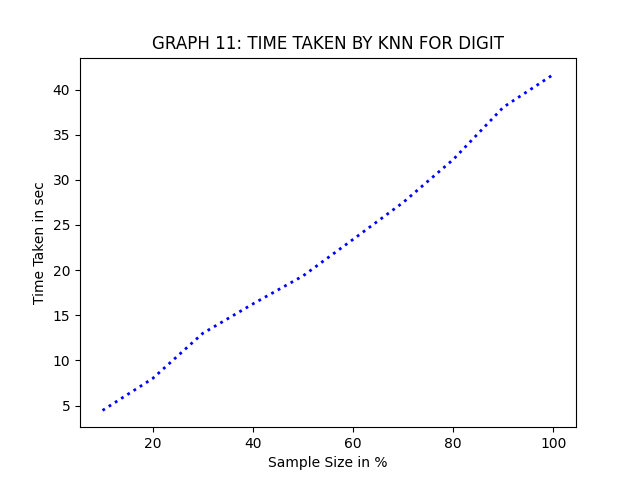
\includegraphics [width = 11cm, height = 8cm]{KNN_TIME_DIGIT.png}
\end {figure}
\begin{center}
\small \textbf {Graph 21:} Time Taken for Digit using kNN\\
\end{center}
\begin{figure} [H]
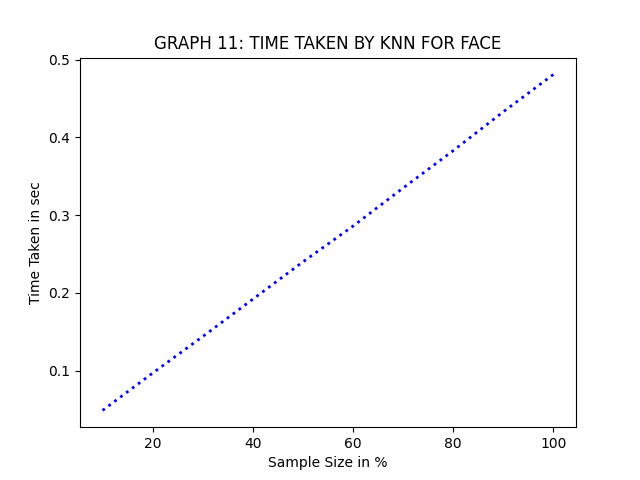
\includegraphics [width = 11cm, height = 8cm]{KNN_TIME_FACE.png}
\end {figure}
\begin{center}
\small \textbf {Graph 22:} Time Taken for Face using kNN\\
\end{center}
\textbullet\ As observed from the graphs, the Time Taken for both face and digit classification has a linear relationship with the sample size. As the sample size increases, the time taken increases.\\ \\
\textbf{iv) Prediction Error}
\begin{figure} [H]
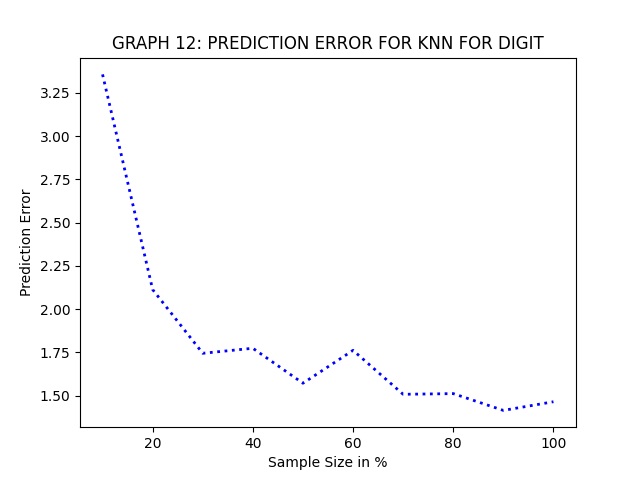
\includegraphics [width = 11cm, height = 8cm]{KNN_PRED_DIGIT.png}
\end {figure}
\begin{center}
\small \textbf {Graph 23:} Prediction Error for Digit using kNN\\
\end{center}
\begin{figure} [H]
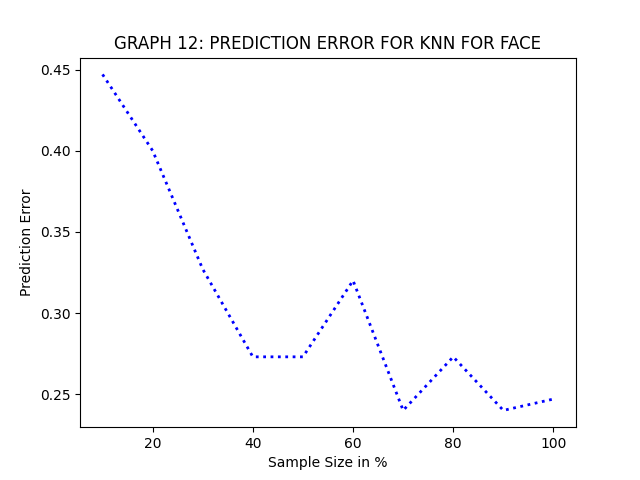
\includegraphics [width = 11cm, height = 8cm]{KNN_PRED_FACE.png}
\end {figure}
\begin{center}
\small \textbf {Graph 24:} Prediction Error for Face using kNN\\
\end{center}
\textbullet\ {As observed from the graphs, the prediction error for Digit is the root mean squared error (RMSE) between the actual test labels and the predicted test labels. As the sample size increases, the prediction error decreases. The prediction error for Face is the ratio of wrong predictions to the total number of predictions. For Face, too, the prediction error decreases as the sample size increases.}
}
\begin{figure} [H]
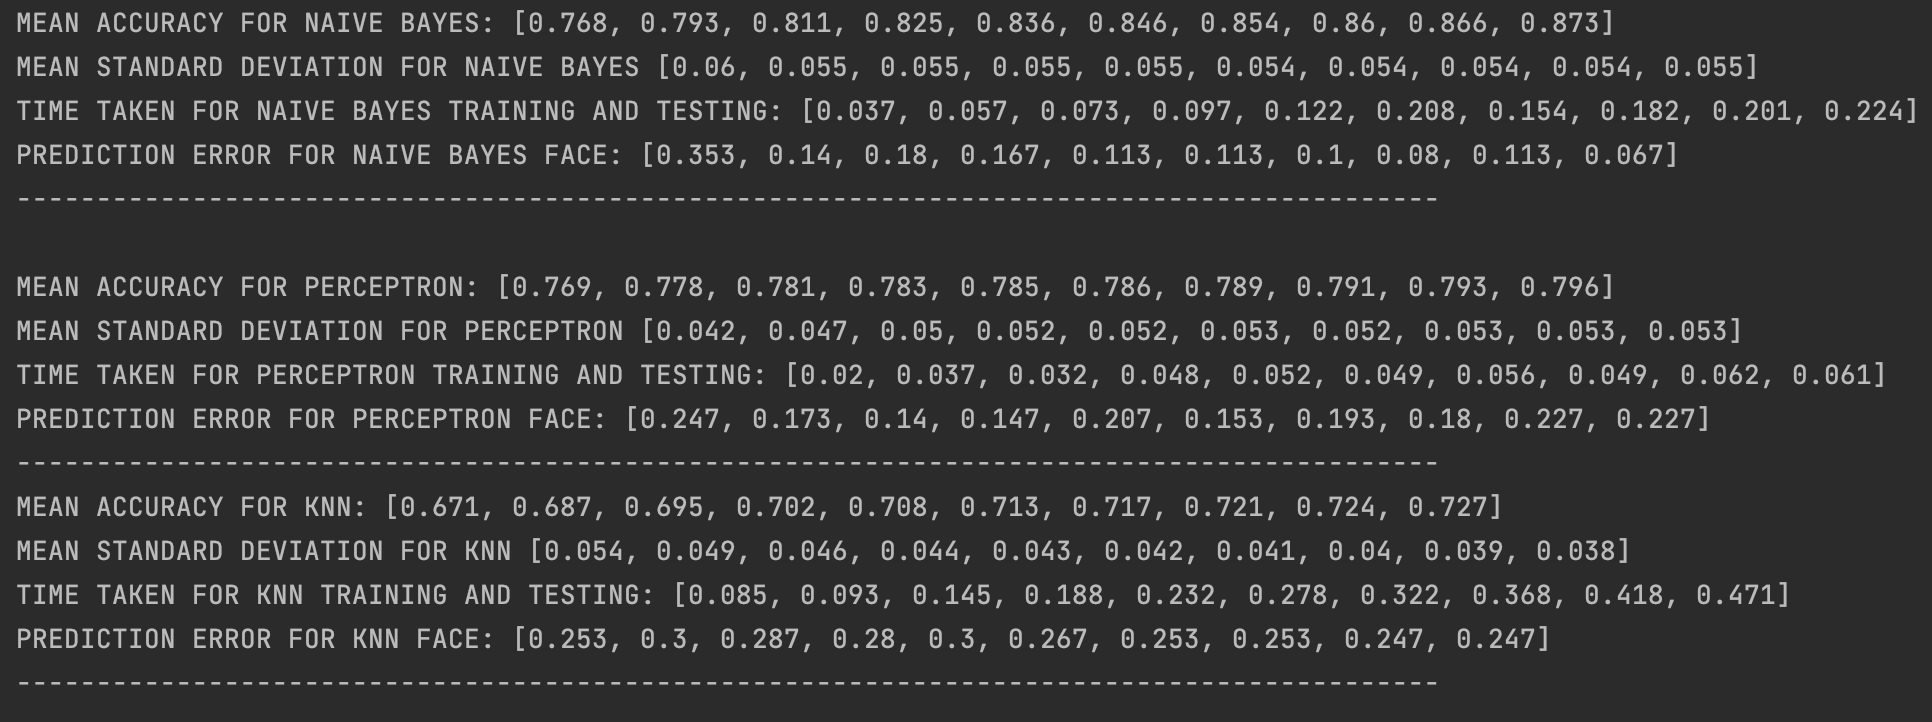
\includegraphics [width = 15cm, height = 5cm]{face.png}
\end {figure}
\begin{center}
\small \textbf {Figure 1:} Output Values for FACE\\
\end{center}
\begin{figure} [H]
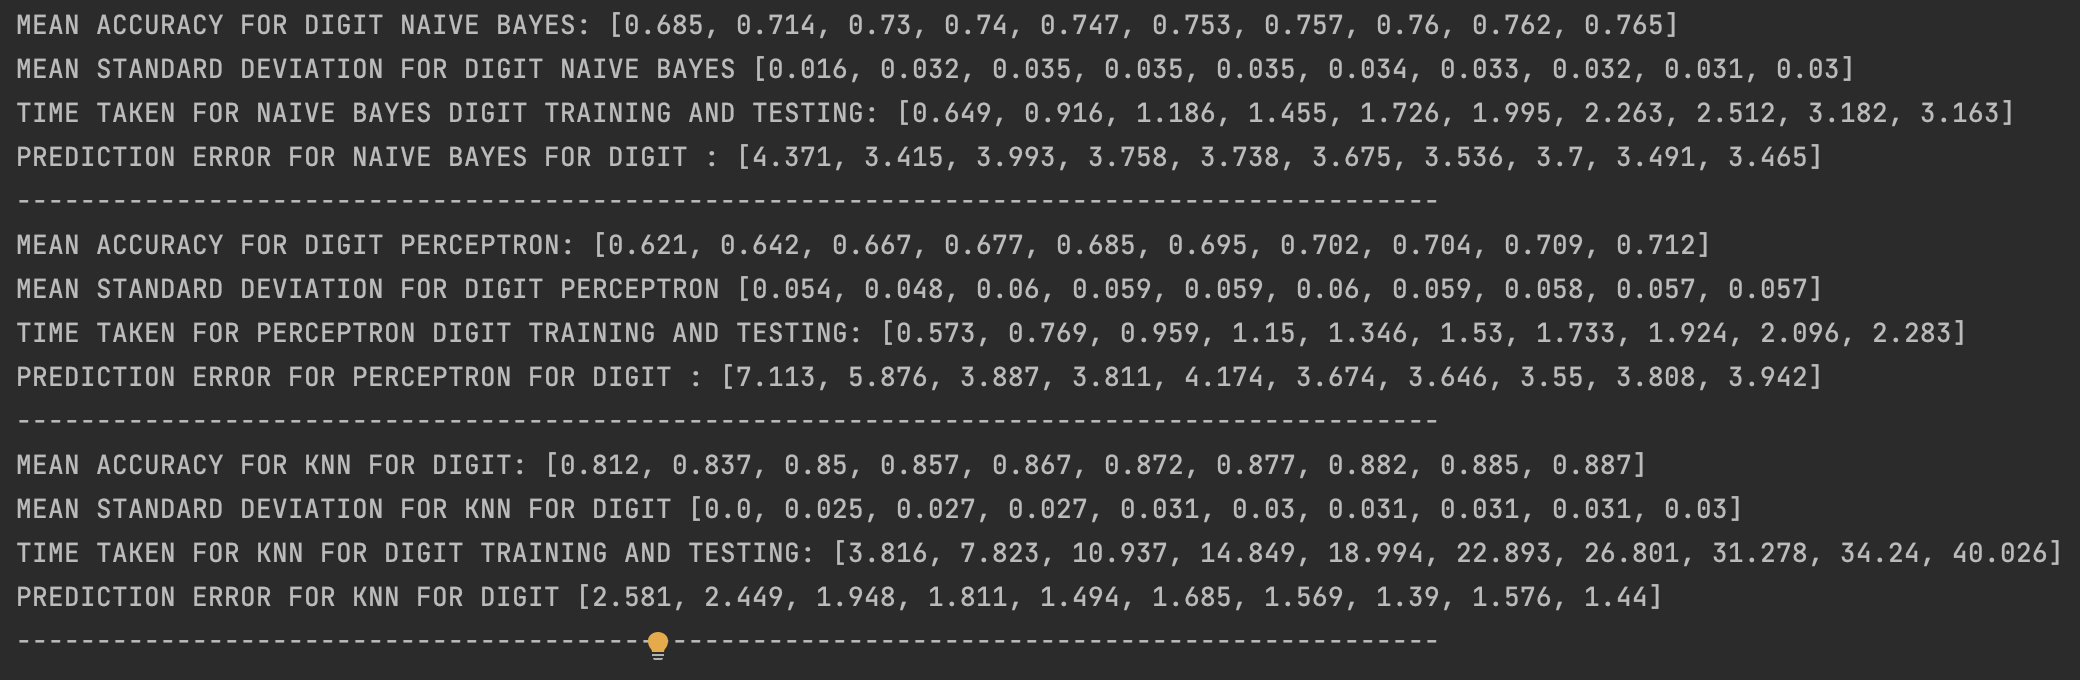
\includegraphics [width = 15cm, height = 5cm]{Digit.png}
\end {figure}
\begin{center}
\small \textbf {Figure 2:} Output Values for DIGIT\\
\end{center}
\end{document}  